\documentclass[tikz, border=2mm]{standalone}
\usepackage{tikz}
\usetikzlibrary{patterns.meta} % Using patterns.meta for better hatching control

\begin{document}
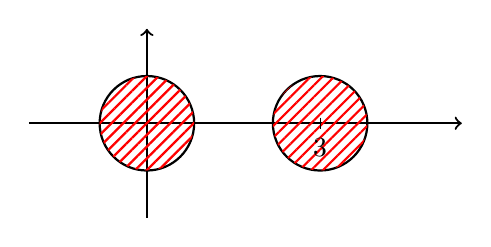
\begin{tikzpicture}

% Define radius for circles
\def\radius{0.6}
% Define pattern style
\tikzset{hatchstyle/.style={
        pattern={Lines[angle=45, distance=3pt, line width=0.8pt]}, % Diagonal lines
        pattern color=red}
        }

% Axes (make them thick like the drawing)
\draw[thick, ->] (-1.5, 0) -- (4, 0); % Horizontal axis
\draw[thick, ->] (0, -1.2) -- (0, 1.2); % Vertical axis

% First Circle (at origin)
\draw[thick] (0,0) circle (\radius);
\fill[hatchstyle] (0,0) circle (\radius);

% Second Circle (to the right)
\coordinate (center2) at (2.2, 0); % Adjust x-coordinate for desired spacing
   
\draw[thick] (center2) circle (\radius);
\fill[hatchstyle] (center2) circle (\radius);

 \draw (2.2, 2pt) -- (2.2, -2pt) node[below] {$3$}; % Tick at u=1

\end{tikzpicture}
\end{document}